\pagenumbering{arabic}
\section{目标简介}
本报告目的是抓取社交媒体平台数据,并进行计算分析,而后对所爬取数据进行分析和可视化展示。

\subsection{数据爬取}
网络爬虫的主要目的是将互联网上的网页下载到本地形成一个或联网内容的镜像备份,通过对内容的解析之后格式化处理进行存储。本报告使用爬虫项目所用框架为scrapy。
\begin{figure}[H]
\centering
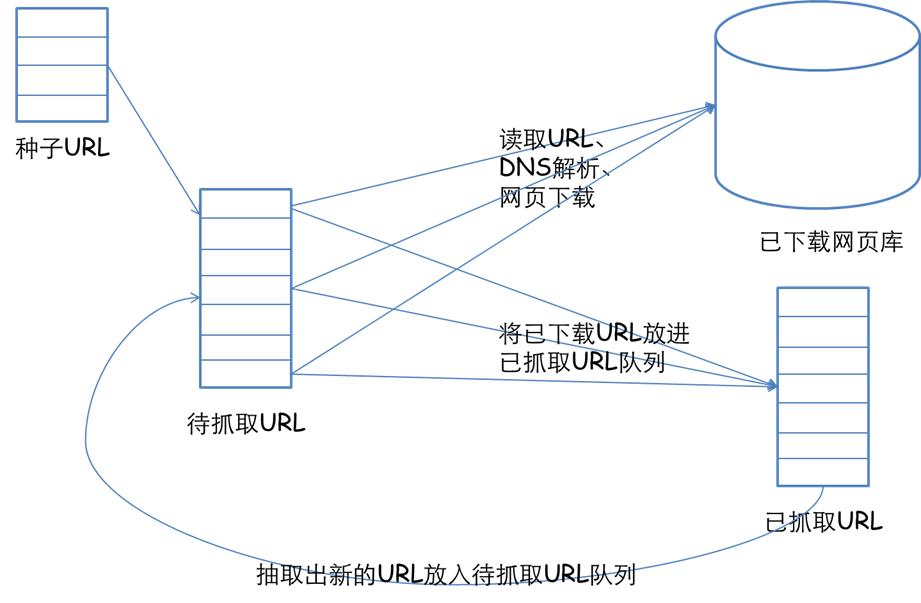
\includegraphics[width=12cm]{figure/spider.png}
\caption{爬虫示意图} \label{fig:spider}
\end{figure}

\subsection{数据分析可视化}
本报告使用pandas、jieba等库进行数据处理,具体方案将在后文阐述。可视化工具使用为pyecharts\ref{fig:pyecharts},可视化数据生成html文件后能够较好实现交互。
\begin{figure}[H]
\centering
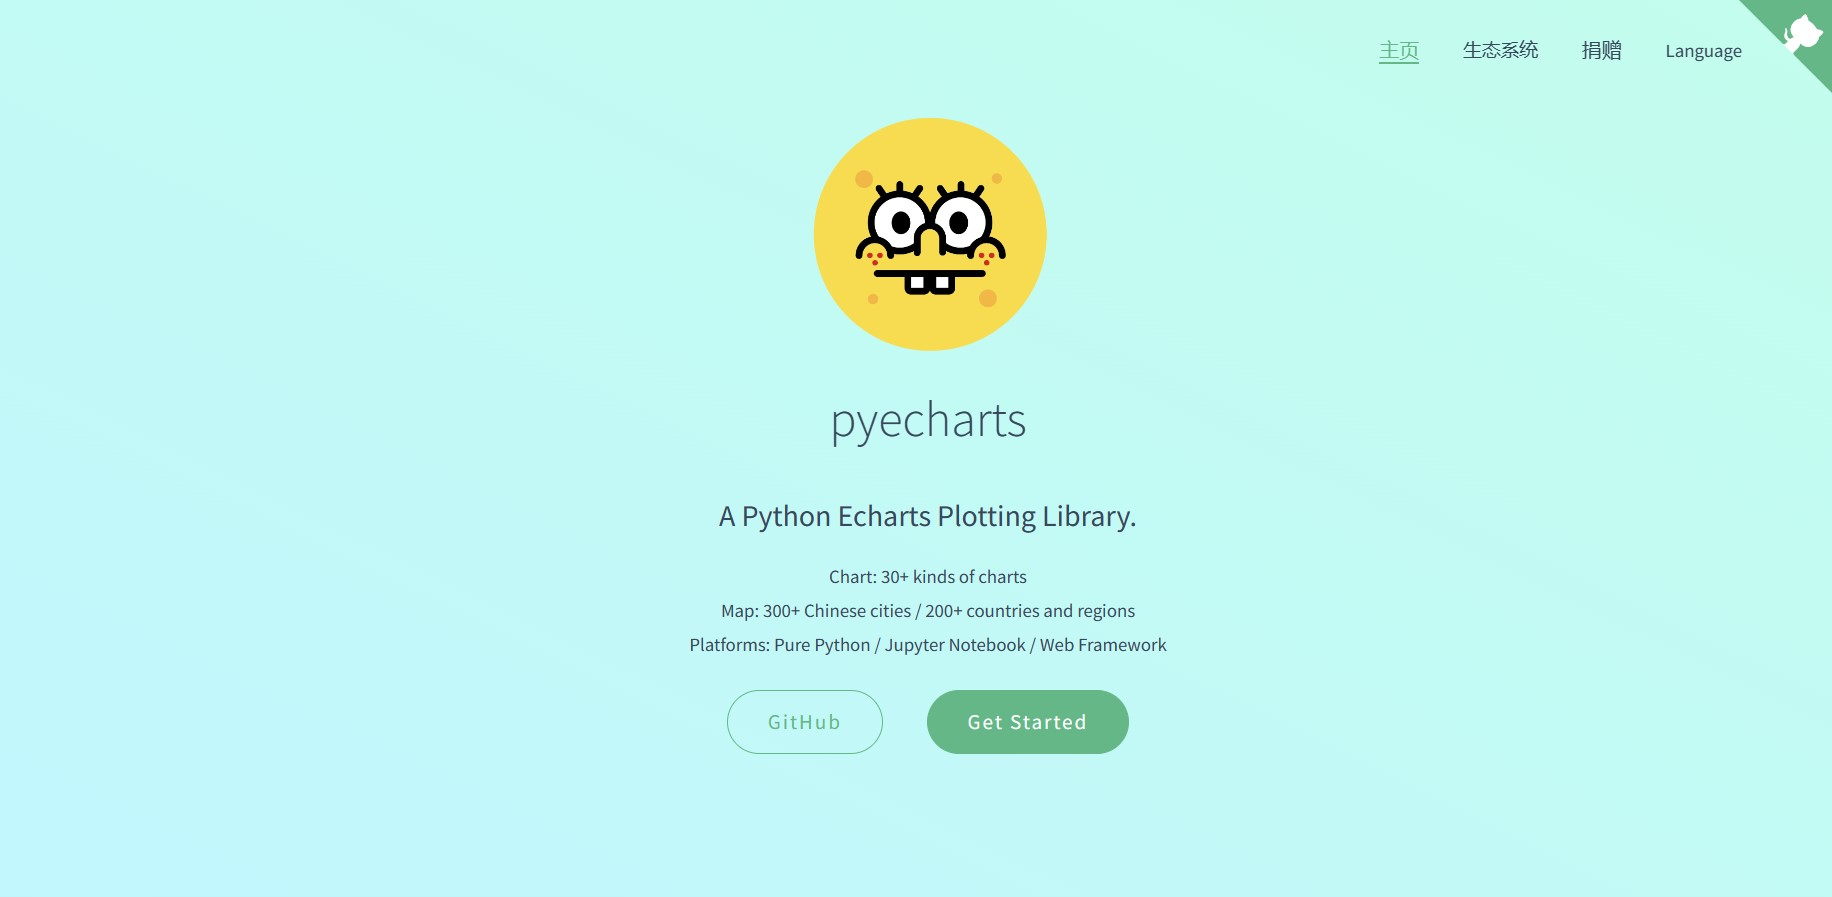
\includegraphics[width=12cm]{figure/pyecharts.jpg}
\caption{pyecharts} \label{fig:pyecharts}
\end{figure}


\subsection{运行环境}
本报告在pycharm(Community Edition 2022.2.2)的windows版本下运行,环境配置为python3.10,界面如图 \ref{fig:pycharm} 所示。
\begin{figure}[H]
\centering
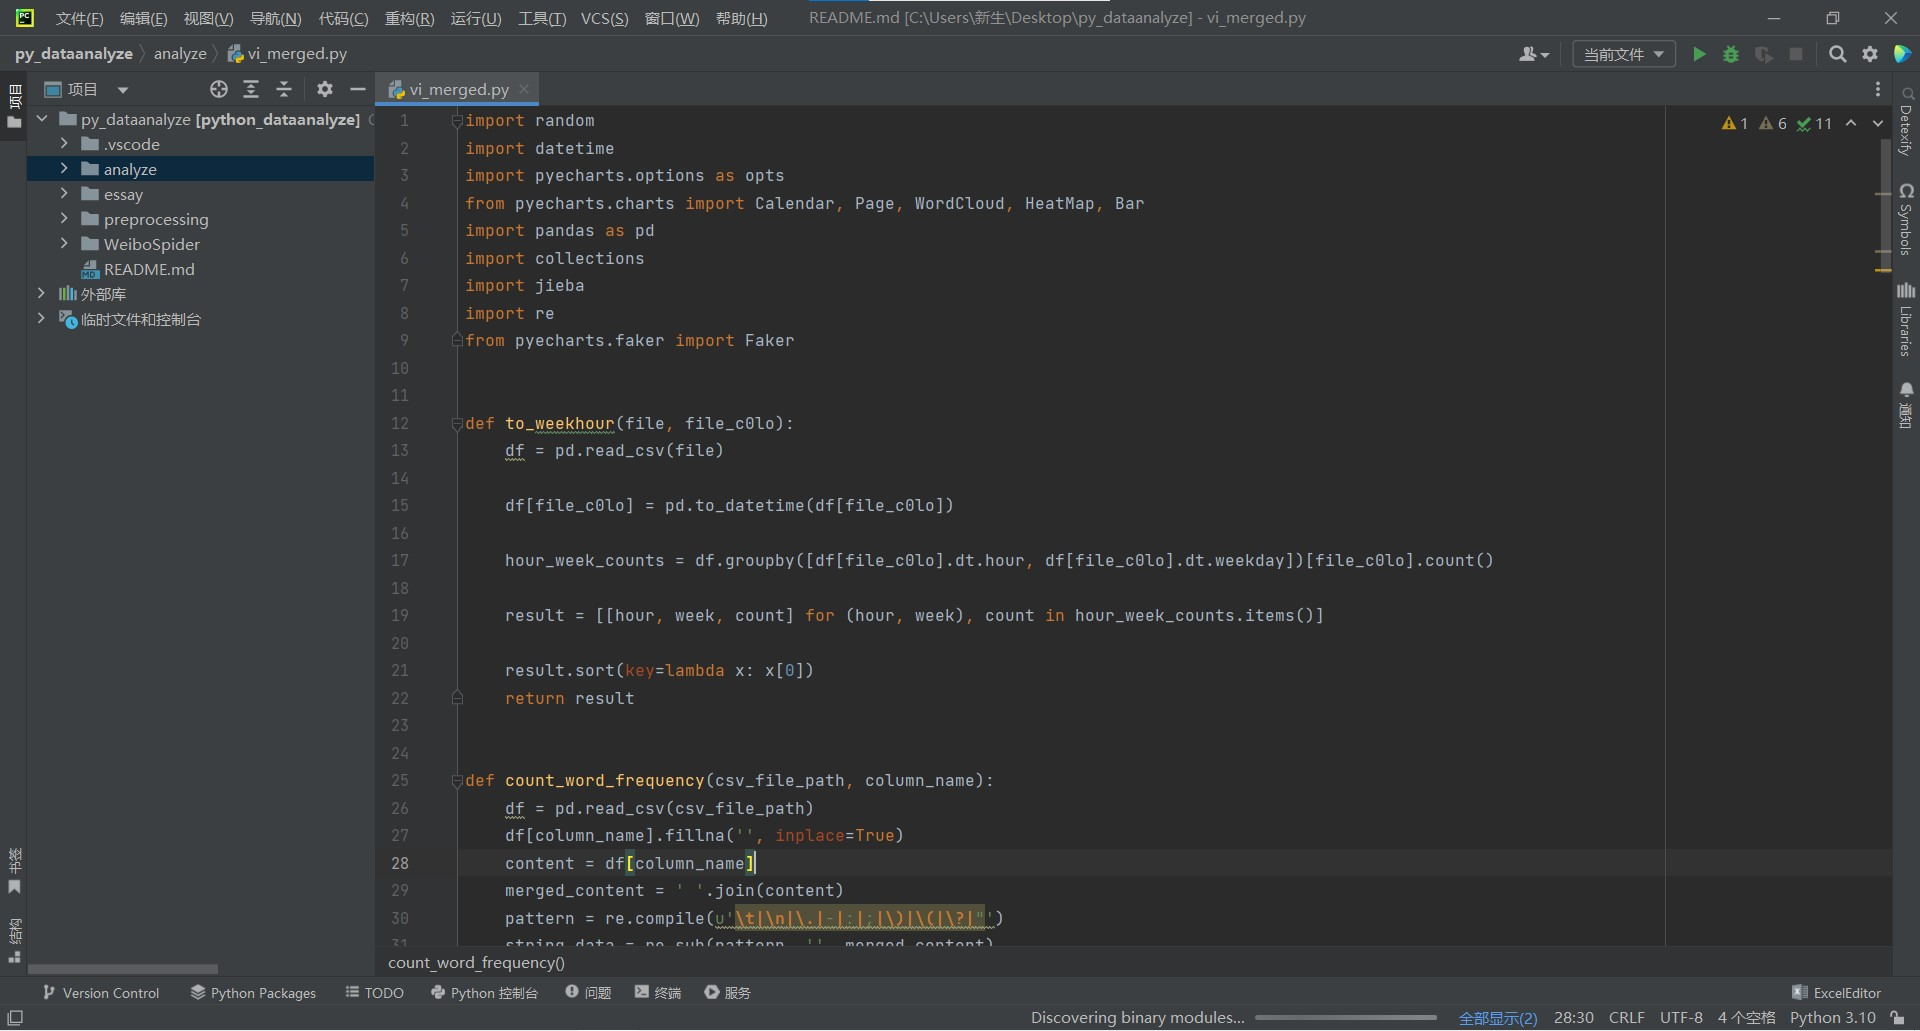
\includegraphics[width=15cm]{figure/environment_pycharm.jpg}
\caption{pycharm运行环境示意图} \label{fig:pycharm}
\end{figure}

